% Logarithmisches Daempfungsdekrement an einer unterdaempften PT2-Sprungantwort
\begin{figure}[!ht]
  \centering
  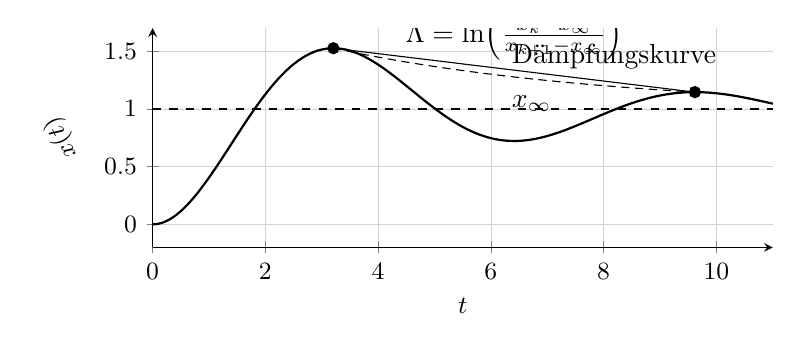
\begin{tikzpicture}
    \pgfmathsetmacro{\damp}{0.2}
    \pgfmathsetmacro{\omegad}{sqrt(1-\damp*\damp)}
    \pgfmathsetmacro{\tpeakone}{pi/\omegad}
    \pgfmathsetmacro{\tpeaktwo}{\tpeakone + 2*pi/\omegad}
    \pgfmathsetmacro{\mpeak}{exp(-\damp*pi/\omegad)}
    \pgfmathsetmacro{\xone}{1 + \mpeak}
    \pgfmathsetmacro{\xtwo}{1 + \mpeak*exp(-2*pi*\damp/\omegad)}
    \begin{axis}[
      width=0.78\textwidth, height=0.36\textwidth,
      grid=both, grid style={line width=.1pt, draw=gray!20},
      major grid style={line width=.2pt, draw=gray!35},
      xlabel={$t$}, ylabel={$x(t)$},
      xmin=0, xmax=11,
      ymin=-0.2, ymax=1.7,
      axis lines=left,
      tick label style={font=\small},
      label style={font=\small},
      trig format=rad
    ]
      \addplot[thick, domain=0:11, samples=400]
        {1 - exp(-\damp*x)*(cos(\omegad*x) + (\damp/\omegad)*sin(\omegad*x))};
      \addplot[dashed] coordinates {(0,1) (11,1)};
      % Daempfungskurve zwischen zwei Maxima (Envelope der Peak-Abstaende)
      \addplot[densely dashed, domain=\tpeakone:\tpeaktwo]
        {1 + \mpeak*exp(-\damp*(x-\tpeakone))};
      \addplot[only marks, mark=*] coordinates {(\tpeakone,\xone) (\tpeaktwo,\xtwo)};
      \draw[->] (axis cs:\tpeakone,\xone) -- (axis cs:\tpeaktwo,\xtwo)
        node[midway, above] {$\Lambda=\ln\!\left(\frac{x_k-x_\infty}{x_{k+1}-x_\infty}\right)$};
      \node[anchor=west] at (axis cs:6.2,1.05) {$x_\infty$};
      \node[anchor=west] at (axis cs:6.2,1.45) {D\"ampfungskurve};
    \end{axis}
  \end{tikzpicture}
  \caption{Unterd\"ampfte PT2-Sprungantwort: Das logarithmische Daempfungsdekrement $\Lambda$ ergibt sich aus zwei aufeinanderfolgenden Maxima der Abweichung von $x_\infty$.}
  \label{fig:log_decrement}
\end{figure}
